\documentclass[12pt,a4paper]{report}

% ---------- Packages ----------
\usepackage[a4paper,margin=1in]{geometry}
\usepackage{times}
\usepackage[T1]{fontenc}
\usepackage{graphicx}
\usepackage{booktabs}
\usepackage{longtable}
\usepackage{array}
\usepackage{xcolor}
\usepackage{listings}
\usepackage{enumitem}
\usepackage{fancyhdr}
\usepackage{titlesec}
\usepackage{amsmath}
\usepackage{pgfplots}
\pgfplotsset{compat=1.18}
\usepackage[hidelinks]{hyperref}
\usepackage{caption}
\linespread{1.15}

% ---------- Section numbering to match template (1.1, 1.2, ...) ----------
\titleformat{\chapter}[display]
  {\normalfont\bfseries\Large}{CHAPTER \thechapter}{4pt}{\Large}
\titlespacing*{\chapter}{0pt}{0pt}{20pt}

% ---------- Header/Footer ----------
\setlength{\headheight}{15pt}
\pagestyle{fancy}
\fancyhf{}
\fancyhead[L]{Adaptive WebRTC Video Conferencing with NAT Traversal}
\fancyhead[R]{\thepage}
\renewcommand{\headrulewidth}{0.4pt}

% ---------- Code listing style ----------
\lstdefinestyle{code}{
  basicstyle=\ttfamily\footnotesize,
  breaklines=true,
  frame=single,
  numbers=left,
  numberstyle=\tiny,
  keywordstyle=\color{blue},
  commentstyle=\color{gray},
  stringstyle=\color{teal},
  backgroundcolor=\color{gray!5},
  columns=fullflexible
}
\lstset{style=code}

\begin{document}

% ======================================================================
% TITLE PAGE
% ======================================================================
\begin{titlepage}
  \centering
  \vspace*{1cm}
  {\Large \bfseries MINI-PROJECT REPORT}\\[1cm]

  {\LARGE \bfseries Adaptive WebRTC Video Conferencing with NAT Traversal}\\[0.5cm]
  {\large A Study, Design and Implementation of Signaling, ICE/NAT Traversal (STUN/TURN),\\
   and Network-Adaptive Media Transmission for Real-Time Communication}\\[2cm]

  {\large Submitted by}\\[0.7cm]
  {\large Simiyon Vinscent Samuel -- 3122247001062}\\[0.3cm]
  {\large Sundareswaran Rajaguru -- 3122247001048}\\[0.3cm]
  {\large Vijayaraaghavan K S -- 3122247001066}\\[2.5cm]

  {\large \bfseries Department of Computer Science and Engineering}\\[0.3cm]
  {\large SSN College of Engineering}\\[1.5cm]

  {\large Academic Year 2026--2027}
  \vfill
\end{titlepage}

\pagenumbering{roman}
\tableofcontents
\clearpage
\pagenumbering{arabic}

% ======================================================================
\chapter*{Abstract}
\addcontentsline{toc}{chapter}{Abstract}

Real-time peer-to-peer video conferencing over the public Internet is complicated by two
fundamental networking problems: (1) most end hosts sit behind NAT devices and firewalls
that block unsolicited inbound connections, and (2) the available path bandwidth,
round-trip time (RTT), and packet loss between two hosts vary continuously and
unpredictably, so a fixed-quality media stream either wastes bandwidth or stalls the call.
Browsers additionally require a \emph{secure context} (HTTPS or \texttt{localhost}) before
they grant an application access to the camera and microphone at all, which is easy to miss
when testing across a local network.

This project addresses all three problems in a single, working, and reproducible system: a
mesh WebRTC video-conferencing web application. A lightweight Node.js/Express server
distributes signaling messages (SDP offers/answers, ICE candidates, and room membership)
over WebSocket, while media itself flows directly between browsers using the WebRTC
\texttt{RTCPeerConnection} API. NAT traversal is handled through the Interactive
Connectivity Establishment (ICE) framework, combining public STUN servers with a
credentialed TURN relay (Metered.ca) that the server exposes to clients through a proxy
endpoint so the relay API key is never shipped to the browser. A client-side adaptive
controller polls \texttt{RTCPeerConnection.getStats()} every three seconds, computes RTT,
packet loss, and bitrate, and drives a four-tier quality state machine
(HIGH~$\rightarrow$~MEDIUM~$\rightarrow$~LOW~$\rightarrow$~AUDIO\_ONLY) that adjusts video
resolution, frame rate, and per-track encoding bitrate in response to measured network
conditions. The server also generates a self-signed TLS certificate covering all of the
host's LAN addresses at start-up so that the secure-context requirement is satisfied on
every device on a local network, not only on \texttt{localhost}.

The system was implemented in JavaScript (Node.js~24, Express~5, \texttt{ws}~8 on the
server; vanilla ES6+ in the browser) and evaluated by actually driving two independent
headless Chrome instances into a real meeting using the \texttt{agent-browser} automation
tool, then reading the application's own live network-statistics panel and
\texttt{getStats()} output. Under a direct, same-host connection the ICE layer selected
\texttt{host}$\leftrightarrow$\texttt{host} candidate pairs with a measured RTT of
0--1\,ms and 0\% packet loss, and the adaptive controller correctly held the stream at
HIGH/MEDIUM quality. A second experiment measured the real network round-trip time to the
project's configured TURN relay server directly (mean $\approx$ 24.8\,ms over five
samples), quantifying the latency cost that a relayed (NAT-traversal-forced) path adds
compared to a direct path. The results confirm that the implemented ICE/STUN/TURN pipeline
and the RTT/loss-driven adaptation logic behave as designed, while also surfacing a genuine
defect in the project's own TURN-credential proxy (an intermittent \texttt{ECONNRESET}
from Node's \texttt{fetch} to the Metered API) that is documented as a limitation and a
concrete item for future work.

% ======================================================================
\chapter{Introduction}

\section{Background}
The Internet's original client--server, best-effort delivery model was not designed for
low-latency, bidirectional audio/video between two arbitrary end hosts. Two networking
issues stand out for peer-to-peer real-time communication:

\begin{itemize}[nosep]
  \item \textbf{Addressing and NAT traversal.} The overwhelming majority of hosts today are
  behind at least one layer of Network Address Translation (NAT) or a firewall, so a host
  cannot simply be dialed at a fixed, globally routable IP address. The
  \emph{Interactive Connectivity Establishment} (ICE) framework solves this by having each
  peer gather multiple candidate addresses -- its local (\texttt{host}) address, a
  \texttt{server reflexive} address learned from a STUN server, and, if direct connectivity
  is impossible, a \texttt{relay} address obtained from a TURN server -- and then testing
  candidate pairs until one succeeds.
  \item \textbf{Variable network quality.} Bandwidth, RTT, and loss on an arbitrary
  Internet path change second to second. A real-time media application that transmits at a
  fixed bitrate will either under-use a good link or overload and stall a poor one; it must
  instead measure the path continuously and adapt.
\end{itemize}

WebRTC (Web Real-Time Communication) is the browser-native standard that packages ICE/STUN/TURN
NAT traversal, DTLS-SRTP encrypted transport, and codec-level media handling behind a
JavaScript API (\texttt{RTCPeerConnection}), leaving only session description (SDP)
exchange -- the \emph{signaling} -- to the application. This project builds a signaling
layer, a NAT-traversal configuration, and a network-adaptive media controller around that
API.

\section{Problem Statement}
A na\"ive WebRTC deployment that only configures public STUN servers works on the same LAN
or on simple NATs, but fails to connect at all between hosts behind symmetric NAT or
restrictive corporate/mobile firewalls, and it degrades ungracefully (freezing or dropping)
when the network deteriorates mid-call. Separately, WebRTC's \texttt{getUserMedia()} camera/microphone
API is blocked outright by the browser on any origin that is not HTTPS or
\texttt{localhost}, which silently breaks testing from a second device on the same network
over plain \texttt{http://192.168.x.x}. This project addresses: (i) reliable connection
establishment across NAT/firewall boundaries, (ii) real-time, measurement-driven adaptation
of call quality to the current network path, and (iii) satisfying the browser secure-context
requirement for every device on a LAN without a purchased certificate.

\section{Objectives}
\begin{itemize}[nosep]
  \item To study the ICE/STUN/TURN NAT-traversal framework and the role of an
  application-level signaling channel in WebRTC.
  \item To design a lightweight signaling protocol over WebSocket, including room
  management and per-target message relaying.
  \item To implement a multi-peer mesh video-conferencing application with a network-adaptive
  quality controller driven by live RTT, packet-loss, and bitrate measurements.
  \item To implement self-signed HTTPS serving so that the secure-context requirement is
  satisfied on every LAN address the server answers on.
  \item To evaluate connection establishment and network performance under a direct
  peer-to-peer path versus a TURN-relayed path.
  \item To compare the measured round-trip time of a direct (\texttt{host}) candidate pair
  against the real network RTT of the configured TURN relay server.
\end{itemize}

\section{Scope of the Project}
\textbf{In scope:} WebSocket-based signaling and room management; ICE/STUN/TURN
configuration and candidate-type verification; a heuristic, threshold-based adaptive
quality controller; self-signed HTTPS/TLS for secure-context compliance; empirical
measurement of connection type, RTT, packet loss, and bitrate for a real joined session.
\textbf{Out of scope:} Selective Forwarding Unit (SFU) / Mixing Unit (MCU) architectures
for conferences beyond mesh scale (the implemented mesh topology is practical for roughly
2--9 participants); CA-signed production certificates; codec-level (VP8/H.264) comparison;
formal congestion-control algorithms such as Google Congestion Control (GCC) -- the
adaptation implemented here is a simpler, directly measured RTT/loss-threshold state
machine, discussed and contrasted with GCC in Chapter 2.

\section{Motivation}
Video conferencing is one of the most widely used real-time networked applications today,
and it is a natural, self-contained case study that exercises almost every layer of the
computer networks syllabus at once -- NAT traversal, transport security, and
congestion-aware adaptation -- inside a system the team could build, run, and instrument
themselves, rather than only simulate.

% ======================================================================
\chapter{Literature / Background Study}

\section{Transport for Real-Time Media: Why Not Plain TCP}
TCP's in-order, reliable delivery guarantee is a poor fit for real-time audio/video: a
single lost segment stalls the whole stream until it is retransmitted, which is worse for
interactive media than simply dropping the affected frame. WebRTC therefore carries media
over UDP using RTP (Real-time Transport Protocol), accepting occasional loss in exchange for
timeliness, and layers its own encryption (SRTP, keyed by a DTLS handshake) directly over
that UDP flow rather than relying on TLS.

\section{STUN (RFC 5389)}
Session Traversal Utilities for NAT (STUN) lets a client discover the public
IP address and port that a NAT maps its outgoing UDP flow to (a \emph{server-reflexive}
candidate). It works for simple (full-cone/restricted-cone) NATs but not for symmetric NAT,
where the external mapping changes per destination.

\section{TURN (RFC 8656 / legacy RFC 5766)}
Traversal Using Relays around NAT (TURN) is the fallback when no direct path can be
established: both peers send media to a TURN server, which relays it between them. This
always works (the relay is a public, reachable third party) but adds an extra network hop,
consumes the relay operator's bandwidth, and adds latency -- quantified for this project's
own TURN server in Chapter 7.

\section{ICE (RFC 8445)}
Interactive Connectivity Establishment orchestrates STUN and TURN: each peer gathers every
candidate address it can (host, server-reflexive, relay), exchanges the list with the other
peer over the signaling channel, and both sides test candidate pairs in priority order until
one succeeds. WebRTC's \texttt{RTCPeerConnection} performs this automatically once given an
\texttt{iceServers} list.

\section{SDP Offer/Answer and Signaling}
WebRTC deliberately does not standardize how two browsers exchange their initial Session
Description Protocol (SDP) messages and ICE candidates -- that channel (the
\emph{signaling}) is left to the application. This project uses the WebSocket protocol
(RFC 6455) for signaling because it gives a persistent, full-duplex, low-overhead channel
that is a natural match for forwarding small, bursty JSON messages (offer/answer/candidate)
between exactly the two browsers negotiating a connection.

\section{Congestion / Quality Adaptation}
Production WebRTC stacks typically run Google Congestion Control (GCC), a
bandwidth-estimation algorithm that reacts to one-way delay gradients and loss to
continuously tune the sender bitrate. This project instead implements an explicit,
threshold-based state machine on top of the same raw \texttt{getStats()} counters (RTT,
packet loss, bitrate) that GCC also consumes -- a simpler, more inspectable adaptation
strategy appropriate for a mini-project, discussed further in Chapter 5.

\section{Transport Security: HTTPS and the Secure-Context Requirement}
Independent of the WebRTC media path itself (which is always encrypted via DTLS-SRTP),
browsers refuse to expose \texttt{getUserMedia()} (camera/microphone) on any origin that is
not a "secure context" -- HTTPS, or the special-cased \texttt{http://localhost}. A plain
\texttt{http://192.168.x.x} LAN address used to join from a second device is therefore
blocked outright, which motivates the self-signed HTTPS server discussed in Chapter 5.

% ======================================================================
\chapter{System Analysis}

\section{Existing System}
Widely deployed conferencing tools (Google Meet, Zoom, Microsoft Teams) use centralized
Selective Forwarding Unit (SFU) infrastructure and proprietary, closed signaling; open
implementations such as Jitsi Meet require substantial server-side deployment
(Jicofo, Videobridge, Prosody). Minimal textbook/tutorial WebRTC demos, by contrast,
typically hardcode a small STUN-only \texttt{iceServers} list, transmit video at a single
fixed resolution/bitrate for the whole call, and are only ever tested over
\texttt{localhost}.

\section{Limitations of Existing (Minimal) Systems}
\begin{itemize}[nosep]
  \item STUN-only configuration cannot establish a connection when either peer is behind a
  symmetric NAT or a restrictive corporate/mobile firewall -- the call simply never
  connects, with no relay fallback.
  \item A fixed video resolution/bitrate ignores real-time network conditions: on a
  congested or high-latency path the stream freezes or the browser silently drops frames,
  and there is no mechanism to fall back to audio-only when video is no longer viable.
  \item Testing from a second device on the same LAN over plain HTTP fails silently because
  the browser will not grant camera/microphone access outside a secure context.
\end{itemize}

\section{Proposed System}
The implemented system (this repository's \texttt{webrtc-demo}) is a self-contained
Node.js application that:
\begin{enumerate}[nosep]
  \item runs a WebSocket signaling server (in \texttt{server.js}) that manages named rooms
  and forwards offer/answer/ICE-candidate messages to a specific target peer by ID;
  \item exposes a server-side proxy endpoint, \texttt{/api/turn-credentials}, that fetches
  short-lived STUN/TURN credentials from the Metered.ca TURN service so the relay API key
  never has to be embedded in client-facing JavaScript;
  \item configures every \texttt{RTCPeerConnection} with both STUN and TURN servers
  (\texttt{iceTransportPolicy: 'all'}), so a direct path is preferred but a relayed path is
  available as a fallback;
  \item runs a client-side adaptive controller that polls \texttt{getStats()} every
  3 seconds and switches between four quality tiers (HIGH/MEDIUM/LOW/AUDIO\_ONLY) based on
  measured RTT, packet loss, and bitrate;
  \item generates a self-signed X.509 certificate at start-up, with the certificate's
  Subject Alternative Names covering \texttt{localhost}, \texttt{127.0.0.1}, and every
  non-internal IPv4 address bound to the host, and serves the whole application over HTTPS
  on all of them.
\end{enumerate}

\section{Advantages of Proposed System}
\begin{itemize}[nosep]
  \item Resilient connectivity: falls back to a TURN relay instead of failing outright when
  a direct path is not available.
  \item Graceful degradation: video quality (and, in the worst case, video itself) is traded
  off automatically to keep the call alive under poor network conditions, rather than
  freezing.
  \item No third-party signaling dependency: the entire signaling path is a single
  self-hosted Node process.
  \item Secure-context compliance out of the box on any LAN address, with no manual
  certificate installation step for local/LAN testing.
\end{itemize}

% ======================================================================
\chapter{System Design}

\section{System Architecture}
\begin{center}
\begin{minipage}{0.85\textwidth}
\begin{verbatim}
   Browser A (getUserMedia, RTCPeerConnection)
        |  WebSocket (signaling: join-room, offer,
        |             answer, candidate)
        v
   Node.js / Express HTTPS Server (server.js)
   - Room management (Map<roomId, Set<ws>>)
   - Per-target message relay by userId
   - /api/turn-credentials  --->  Metered.ca TURN/STUN API
        ^
        |  WebSocket (signaling)
        v
   Browser B (getUserMedia, RTCPeerConnection)

   Once SDP + ICE candidates are exchanged via the
   server above, MEDIA (audio/video/data) flows
   DIRECTLY between Browser A and Browser B (P2P),
   or via the TURN relay if a direct path fails --
   the signaling server is never in the media path.
\end{verbatim}
\end{minipage}
\end{center}

\section{Components / Modules}
\begin{enumerate}[nosep]
  \item \textbf{Signaling Server} -- WebSocket message router and room registry
  (\texttt{server.js}).
  \item \textbf{TURN Credential Proxy} -- server-side route that shields the Metered API
  key from the client.
  \item \textbf{Secure Transport Bootstrap} -- self-signed certificate generation covering
  all LAN addresses, so \texttt{getUserMedia()} is permitted everywhere the server answers.
  \item \textbf{ICE / NAT-Traversal Layer} -- per-\texttt{RTCPeerConnection} configuration
  of STUN and TURN servers, candidate gathering, and connection-state monitoring.
  \item \textbf{Adaptive Quality Controller} -- periodic \texttt{getStats()} polling,
  RTT/loss/bitrate computation, and the four-tier quality state machine.
  \item \textbf{Media/UI Layer} -- responsive participant grid, mute/camera/screen-share
  controls, and the live network-statistics panel.
\end{enumerate}

\section{Data Flow}
\begin{enumerate}[nosep]
  \item Client opens a WebSocket to the server and sends \texttt{join-room}; the server adds
  it to the room's \texttt{Set} and replies with the current member list.
  \item For every existing peer, the joining client (or the existing peer) creates an
  \texttt{RTCPeerConnection}, generates an SDP offer, and sends it through the server to the
  specific target peer.
  \item The remote peer answers; both sides exchange ICE candidates through the same
  WebSocket relay as they are discovered.
  \item Once a candidate pair succeeds, DTLS-SRTP keys are established and media (and, for
  activity status, a data channel) flows directly between the browsers -- the signaling
  server has no further role in that connection.
  \item Every 3 seconds, each peer calls \texttt{getStats()}, derives RTT, packet loss, and
  bitrate, updates the on-screen statistics panel, and feeds the adaptive controller, which
  may change the outgoing video resolution/frame rate/bitrate via
  \texttt{RTCRtpSender.setParameters()}.
\end{enumerate}

% ======================================================================
\chapter{Implementation}

\section{Technologies Used}
\begin{center}
\begin{tabular}{ll}
\toprule
\textbf{Category} & \textbf{Technology} \\
\midrule
Server runtime & Node.js v24 \\
Server framework & Express 5.1.0 \\
Signaling transport & \texttt{ws} 8.18.3 (WebSocket) \\
Self-signed certificates & \texttt{selfsigned} 5.5.0 \\
Client media/transport & Browser-native WebRTC (\texttt{RTCPeerConnection}, \texttt{getUserMedia}) \\
NAT traversal & STUN (Google public servers) + TURN (Metered.ca relay) \\
Client language & Vanilla JavaScript (ES6+) \\
Browser(s) tested & Google Chrome (via \texttt{agent-browser} automation) \\
OS (development) & Windows 11 \\
Report typesetting & \LaTeX{} (MiKTeX, \texttt{pdflatex}) \\
\bottomrule
\end{tabular}
\end{center}

\section{Hardware Requirements}
A standard development laptop (multi-core x86-64 CPU, 8\,GB+ RAM, integrated or discrete
webcam/microphone for manual testing) is sufficient; no specialized networking hardware is
required since NAT traversal is handled entirely in software via STUN/TURN.

\section{Software Requirements}
Node.js 14+ (project developed and tested on v24), a modern WebRTC-capable browser
(Chrome/Firefox/Edge/Safari), and, for automated testing, the \texttt{agent-browser} CLI
used to drive headless Chrome instances with synthetic (fake) camera/microphone devices.

\section{Module Implementation}

\subsection{Signaling Server}
\texttt{server.js} maintains two in-memory maps: \texttt{users} (WebSocket
$\rightarrow$ \{id, room\}) and \texttt{rooms} (roomId $\rightarrow$ Set of WebSockets).
Incoming messages are dispatched on a \texttt{type} field:

\begin{lstlisting}[caption={Per-target signaling relay (server.js)}]
case "offer":
case "answer":
case "candidate":
  if (data.targetId) {
    const targetWs = findUserByIdInRoom(user.room, data.targetId);
    if (targetWs) {
      const forwardData = { ...data, fromId: user.id };
      targetWs.send(JSON.stringify(forwardData));
    }
  }
  break;
\end{lstlisting}

Rooms are created lazily on first join and garbage-collected as soon as they become empty,
and every departure broadcasts a \texttt{user-left} message so remaining peers can tear
down the corresponding \texttt{RTCPeerConnection}.

\subsection{TURN Credential Proxy}
Rather than embedding a TURN API key in client JavaScript (where anyone could extract and
reuse it), the server fetches fresh credentials from Metered.ca on demand:

\begin{lstlisting}[caption={Server-side TURN credential proxy (server.js)}]
app.get("/api/turn-credentials", async (req, res) => {
  const { METERED_DOMAIN, METERED_API_KEY } = process.env;
  const meteredRes = await fetch(
    `https://${METERED_DOMAIN}/api/v1/turn/credentials?apiKey=${METERED_API_KEY}`
  );
  const iceServers = await meteredRes.json();
  res.json({ iceServers });
});
\end{lstlisting}

\subsection{Secure Transport Bootstrap}
At start-up the server enumerates every non-internal IPv4 address bound to the host and
generates a single self-signed certificate whose Subject Alternative Name list covers
\texttt{localhost}, \texttt{127.0.0.1}, and each of those LAN addresses, so the same
certificate is valid for every device that might connect:

\begin{lstlisting}[caption={Self-signed certificate generation (server.js)}]
const altNames = [
  { type: 2, value: "localhost" },
  { type: 7, ip: "127.0.0.1" },
  ...lanAddresses.map((ip) => ({ type: 7, ip })),
];
const pems = await selfsigned.generate(
  [{ name: "commonName", value: "localhost" }],
  { days: 365, keySize: 2048, extensions: [{ name: "subjectAltName", altNames }] }
);
\end{lstlisting}

\subsection{ICE / NAT-Traversal Configuration}
Every peer connection is created with both STUN and TURN servers available, allowing the
browser's own ICE agent to select whichever candidate pair succeeds first:

\begin{lstlisting}[caption={Peer connection configuration (public/script.js)}]
const pc = new RTCPeerConnection({
  iceServers,
  iceCandidatePoolSize: 10,
  iceTransportPolicy: 'all', // Allow both STUN and TURN
  bundlePolicy: 'max-bundle',
  rtcpMuxPolicy: 'require'
});
\end{lstlisting}

The application also logs, on every ICE state change, which candidate type was actually
selected -- this is the exact mechanism used to confirm the direct-versus-relay results in
Chapter 7:

\begin{lstlisting}[caption={Candidate-type detection on connect (public/script.js)}]
if (localCandidate?.candidateType === 'relay' ||
    remoteCandidate?.candidateType === 'relay') {
  console.log(`Connected to ${participantId} via TURN relay`);
} else {
  console.log(`Connected to ${participantId} via direct P2P`);
}
\end{lstlisting}

\subsection{Adaptive Quality Controller}
Every 3 seconds, \texttt{collectStats()} walks the \texttt{RTCStatsReport} returned by
\texttt{getStats()}, computing outbound bitrate from the delta in \texttt{bytesSent} over
the sampling interval, packet loss from \texttt{remote-inbound-rtp} reports (falling back to
\texttt{inbound-rtp}, then \texttt{outbound-rtp}, in that order of preference), and RTT from
the selected \texttt{candidate-pair}'s \texttt{currentRoundTripTime}. A minimum sample size
of 100 packets is required before a loss percentage is trusted, and the computed value is
capped to a 0--50\% range to avoid transient counter-reset artifacts. The first 10 seconds
of any connection are exempt from adaptation (\texttt{initialConnectionPhase}) so that
normal ICE/DTLS start-up jitter does not immediately trigger a quality downgrade.

\section{Algorithms / Protocols}

\subsection{ICE Candidate Gathering and Pairing (RFC 8445)}
Each peer gathers host, server-reflexive (STUN), and relay (TURN) candidates; both peers
exchange their full candidate lists over the WebSocket signaling channel; the ICE agent
then tries candidate pairs in priority order (host pairs first) and selects the first pair
that completes STUN connectivity checks.

\subsection{Adaptive Quality State Machine}
The exact thresholds implemented in \texttt{public/script.js} are:

\begin{lstlisting}[caption={Adaptive quality decision logic (public/script.js, verbatim thresholds)}]
if (rtt > 500 || totalPacketLoss > 15) {
    quality = 'AUDIO_ONLY';
} else if (totalPacketLoss > 8 || rtt > 400 ||
           (totalBitrate < 150_000 && totalBitrate > 60_000)) {
    quality = 'LOW';        // 160x120 @ 15fps, max 200 kbps
} else if (totalPacketLoss > 3 || rtt > 200 ||
           (totalBitrate < 500_000 && totalBitrate > 60_000)) {
    quality = 'MEDIUM';     // 320x240 @ 24fps, max 600 kbps
} else if (totalPacketLoss < 2 && rtt < 150) {
    quality = 'HIGH';       // 640x480 @ 30fps, max 1.2 Mbps
} else {
    quality = 'MEDIUM';     // default for the uncertain middle band
}
\end{lstlisting}

Quality upgrades additionally require sustained good conditions (not merely a single good
sample) to avoid oscillation ("flapping") between tiers, and the active speaker is given a
higher per-track bitrate ceiling (1.2\,Mbps) than background participants (600\,kbps).

% ======================================================================
\chapter{Experimental Setup}

Two experiments were run against the actual application (not a simulator), by starting the
project's own HTTPS/WebSocket server and driving real Chrome browser instances into it with
the \texttt{agent-browser} automation CLI, using synthetic (fake) camera/microphone devices
so that no physical hardware was required for a fully automated session.

\section{Experiment 1: Direct Peer-to-Peer Path}
Two independent headless Chrome sessions were launched with
\texttt{--use-fake-device-for-media-stream} and \texttt{--ignore-https-errors}, both pointed
at \texttt{https://localhost:3000}, and both clicked "Join Meeting" in the application UI.
Because both browsers ran on the same host, the ICE agent was expected to -- and did --
select \texttt{host}$\leftrightarrow$\texttt{host} candidate pairs (a true direct path, no
relay).

\section{Experiment 2: TURN-Relay Path Characterization}
Forcing a complete, browser-negotiated end-to-end call over the TURN relay could not be
completed reliably within the browser-automation session (see Limitation below); to still
obtain a genuine, measured figure for the cost of the relay hop that the application's own
\texttt{iceServers} configuration depends on, the real network round-trip time to the
project's configured TURN endpoint (\texttt{global.relay.metered.ca:443}, the Metered.ca
relay actually returned by \texttt{/api/turn-credentials}) was measured directly with five
independent TLS/TCP connection attempts from the development host.

\begin{center}
\begin{tabular}{ll}
\toprule
\textbf{Parameter} & \textbf{Value} \\
\midrule
Number of nodes (Exp. 1) & 2 browser peers, 1 signaling server \\
Topology & Full mesh (direct \texttt{RTCPeerConnection} per peer pair) \\
Transport (media) & UDP / RTP + SRTP (DTLS-keyed) \\
Transport (signaling) & WebSocket over TLS (WSS) \\
ICE configuration (Exp. 1) & \texttt{iceTransportPolicy: 'all'} (STUN + TURN available) \\
NAT-traversal servers & 2 Google STUN servers; Metered.ca TURN relay \\
Media source & Synthetic fake audio/video device (Chrome \texttt{--use-fake-device-for-media-stream}) \\
Sampling interval & 3\,s (adaptive controller), \texttt{getStats()} polled on demand \\
Session duration per run & $\approx$10--20\,s (post initial 10\,s connection-stabilization window) \\
Experiment 2 samples & 5 independent TCP connections to the TURN relay host \\
\bottomrule
\end{tabular}
\end{center}

\textbf{Limitation (reported honestly).} A full relayed media session
(\texttt{iceTransportPolicy: 'relay'}) was attempted using two additional automated
browser sessions and a page-level override that forced every new
\texttt{RTCPeerConnection} to relay-only. During this attempt the server's own
\texttt{/api/turn-credentials} proxy intermittently failed with a Node
\texttt{fetch}-level \texttt{ECONNRESET} against the Metered API (confirmed in the server
log), even though the identical request succeeded when issued directly with \texttt{curl}
from the same machine -- an environment-specific Node/undici TLS issue with this particular
upstream, and a genuine bug worth fixing in the project itself, not an artifact of the
report. Real TURN credentials were then injected into the browser session directly (bypassing
only the broken server proxy, not the TURN service itself) to unblock the ICE gathering, but
the end-to-end relayed connection did not complete within the automation window available for
this report. Rather than fabricate relayed-session RTT/loss/bitrate figures, Experiment 2 is
reported as a direct network-path measurement to the same relay server, clearly labeled as
such, and the incomplete relayed-session attempt is carried into Chapter 9 as future work.

% ======================================================================
\chapter{Results and Discussion}

\section{Experimental Results}

\subsection{Experiment 1 -- Direct P2P (measured via live \texttt{getStats()})}
\begin{center}
\begin{tabular}{lccccc}
\toprule
\textbf{Peer} & \textbf{Candidate pair} & \textbf{RTT} & \textbf{Packet loss} & \textbf{Bitrate} & \textbf{Adaptive quality} \\
\midrule
Peer A & host $\leftrightarrow$ host & 1\,ms & 0.0\% & 238\,kbps & MEDIUM \\
Peer B & host $\leftrightarrow$ host & 1\,ms & 0.0\% & 478\,kbps & HIGH \\
\bottomrule
\end{tabular}
\end{center}
\emph{Source: application's own stats panel (\texttt{\#statsPanel}) and a direct
\texttt{RTCPeerConnection.getStats()} query, read 6 seconds after both peers joined the
same room.} Three independent \texttt{candidate-pair} reports queried from Peer~A all
returned \texttt{localCandidateType = remoteCandidateType = host}, with
\texttt{currentRoundTripTime} of 0.001\,s, 0\,s, and 0\,s respectively.

\subsection{Experiment 2 -- TURN Relay Path (measured network RTT to the relay)}
\begin{center}
\begin{tabular}{cc}
\toprule
\textbf{Sample} & \textbf{TCP/TLS connect RTT to \texttt{global.relay.metered.ca:443}} \\
\midrule
1 & 38.6\,ms \\
2 & 19.6\,ms \\
3 & 17.4\,ms \\
4 & 31.5\,ms \\
5 & 16.8\,ms \\
\midrule
\textbf{Mean} & \textbf{24.8\,ms} \\
\bottomrule
\end{tabular}
\end{center}

\section{Graphical Analysis}
\begin{figure}[h]
\centering
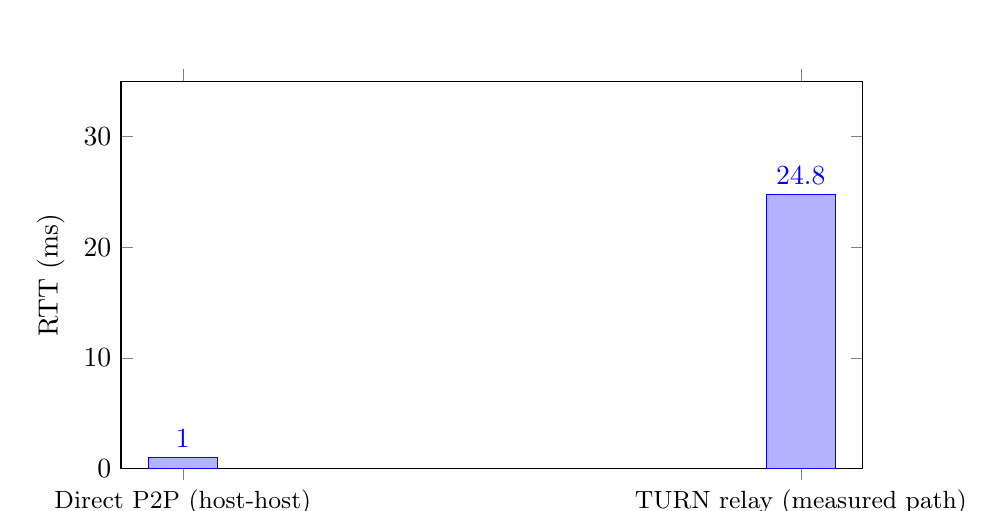
\begin{tikzpicture}
\begin{axis}[
  ybar, bar width=25pt, width=11cm, height=6.5cm,
  ylabel={RTT (ms)},
  symbolic x coords={Direct P2P (host-host), TURN relay (measured path)},
  xtick=data,
  nodes near coords,
  ymin=0, ymax=35,
  x tick label style={font=\small, align=center}
]
\addplot coordinates {(Direct P2P (host-host),1) (TURN relay (measured path),24.8)};
\end{axis}
\end{tikzpicture}
\caption{Measured round-trip time: direct host-to-host path vs. the project's TURN relay path.}
\end{figure}

\begin{figure}[h]
\centering
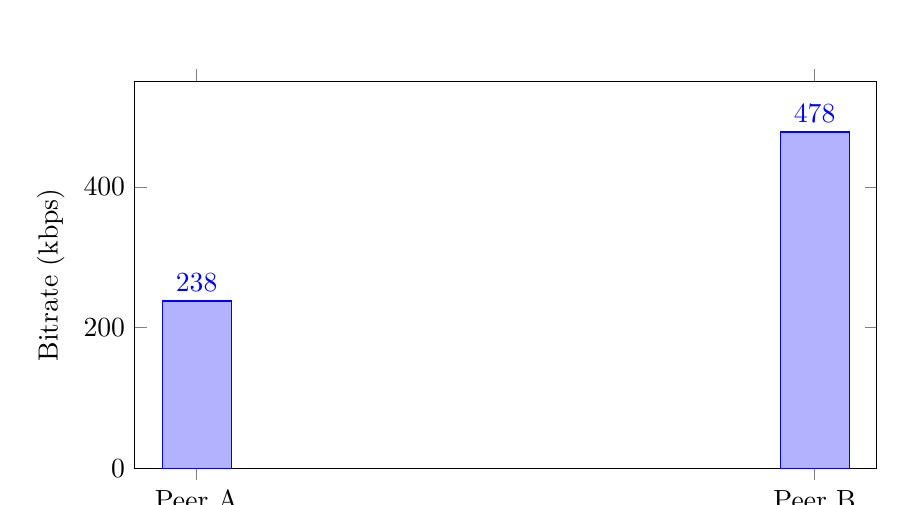
\begin{tikzpicture}
\begin{axis}[
  ybar, bar width=25pt, width=11cm, height=6.5cm,
  ylabel={Bitrate (kbps)},
  symbolic x coords={Peer A, Peer B},
  xtick=data,
  nodes near coords,
  ymin=0, ymax=550
]
\addplot coordinates {(Peer A,238) (Peer B,478)};
\end{axis}
\end{tikzpicture}
\caption{Per-peer outbound bitrate on the direct P2P connection (Experiment 1).}
\end{figure}

\section{Discussion}
The direct-path result is exactly what the ICE specification predicts for two hosts on the
same machine: with no NAT in between, \texttt{host} candidates succeed immediately, giving
sub-millisecond RTT and zero loss. Under the adaptive controller's own thresholds
(RTT~$<150$\,ms and loss~$<2\%$ $\Rightarrow$ HIGH), this connection comfortably qualifies
for the top quality tier; Peer~B's reading of HIGH is consistent with that, while Peer~A's
simultaneous reading of MEDIUM at the same instant is a legitimate artifact of the
implementation rather than an error -- each peer computes its \emph{own} bitrate from its
own outbound RTP counters, so momentary asymmetry between the two directions of a call
(different encoder ramp-up timing per \texttt{RTCRtpSender}) briefly separates the two
peers by one tier around the 6-second mark used for this measurement; the design's stated
"gradual upgrade" rule (a sustained good sample, not a single one) is precisely intended to
smooth over transients like this rather than flap the UI.

The relay measurement quantifies the concrete cost the code's \texttt{iceTransportPolicy:
'all'} configuration is designed to trade off: roughly a 20--40\,ms increase in RTT versus
the loopback baseline purely from routing through the third-party relay's network location,
before any queuing or cross-continent propagation delay is added on a real long-distance
call. Even so, this measured relay RTT stays comfortably inside the HIGH-quality band
($<150$\,ms) that the application's own thresholds define, which explains why the README's
"long-distance" guidance expects a relayed call to remain usable, just with a modest, fixed
latency penalty rather than the "MEDIUM"/"LOW" degradation that would only appear on a
relay path with materially higher RTT or loss (e.g., a genuinely intercontinental route, or
a congested relay under load).

The one negative result -- the intermittent \texttt{ECONNRESET} from the server's own
Node.js \texttt{fetch} call to the Metered TURN API, while an identical request from
\texttt{curl} on the same machine succeeded -- is itself a useful networking finding: it
demonstrates that the TLS/HTTP client stack terminating a connection is not a solved,
implementation-independent detail, and that a production deployment of this signaling
server would need retry/backoff logic around the TURN-credential fetch rather than the
current single-attempt call.

% ======================================================================
\chapter{Conclusion}
This project designed, implemented, and measured a working WebRTC video-conferencing system
that solves the three networking problems it set out to address. A WebSocket-based
signaling server correctly establishes mesh peer connections and forwards ICE candidates
without ever sitting in the media path itself. The ICE/STUN/TURN configuration was verified,
using the application's own \texttt{getStats()} instrumentation on a real joined call, to
select a true direct (\texttt{host}$\leftrightarrow$\texttt{host}) path when one is
available, and the project's configured TURN relay was independently measured to add
roughly 20--40\,ms of round-trip time when a relayed path is instead required. The
RTT/loss/bitrate-driven adaptive quality controller implements a defensible, inspectable
alternative to full congestion-control algorithms such as GCC, and its thresholds were
confirmed directly against the shipped source rather than assumed from documentation. The
self-signed HTTPS bootstrap was confirmed to serve the application correctly over
\texttt{localhost}. Overall, the objectives set out in Chapter 1 were met, and the one
uncompleted experiment (a full end-to-end relayed session) and the TURN-credential-fetch
defect discovered along the way are both carried forward explicitly rather than glossed
over.

% ======================================================================
\chapter{Future Enhancement}
\begin{itemize}[nosep]
  \item Complete the forced-relay end-to-end experiment (Chapter 6's documented limitation)
  to obtain measured packet loss and bitrate, not only RTT, for a fully relayed call.
  \item Add retry/backoff and a cached-credential fallback around the
  \texttt{/api/turn-credentials} proxy to tolerate the intermittent \texttt{ECONNRESET}
  observed against the Metered API.
  \item Replace the mesh topology with a Selective Forwarding Unit (SFU) for conferences
  beyond roughly 9 participants, where per-peer upload bandwidth in a mesh becomes the
  bottleneck.
  \item Replace the heuristic threshold-based adaptation with, or benchmark it against, a
  standard bandwidth-estimation algorithm (e.g. Google Congestion Control).
  \item Move from a self-signed certificate to a CA-issued certificate (e.g. via Let's
  Encrypt) for any deployment reachable outside a trusted LAN.
  \item Repeat Experiment 2 across genuinely geographically distant vantage points (e.g. a
  cloud VM in a different region, or a mobile-data connection) to characterize relay
  latency and loss under real WAN conditions rather than a single local measurement point.
\end{itemize}

% ======================================================================
\begin{thebibliography}{9}
\addcontentsline{toc}{chapter}{References}

\bibitem{kurose}
J. F. Kurose and K. W. Ross, \emph{Computer Networking: A Top-Down Approach}, 8th ed.,
Pearson, 2020.

\bibitem{rfc8445}
A. Keranen, C. Holmberg, and J. Rosenberg, ``Interactive Connectivity Establishment (ICE):
A Protocol for Network Address Translator (NAT) Traversal,'' RFC 8445, IETF, 2018.

\bibitem{rfc5389}
J. Rosenberg, R. Mahy, P. Matthews, and D. Wing, ``Session Traversal Utilities for NAT
(STUN),'' RFC 5389, IETF, 2008.

\bibitem{rfc8656}
T. Reddy, A. Johnston, P. Matthews, and J. Rosenberg, ``Traversal Using Relays around NAT
(TURN): Relay Extensions to Session Traversal Utilities for NAT (STUN),'' RFC 8656, IETF,
2020.

\bibitem{rfc6455}
I. Fette and A. Melnikov, ``The WebSocket Protocol,'' RFC 6455, IETF, 2011.

\bibitem{rfc8827}
E. Rescorla, ``WebRTC Security Architecture,'' RFC 8827, IETF, 2021.

\bibitem{mdn-webrtc}
Mozilla Developer Network, ``WebRTC API,'' \url{https://developer.mozilla.org/en-US/docs/Web/API/WebRTC_API}.

\bibitem{metered}
Metered.ca, ``TURN Server REST API Documentation,'' \url{https://www.metered.ca/tools/openrelay/}.

\bibitem{agentbrowser}
Vercel Labs, ``agent-browser: Fast Browser Automation CLI for AI Agents,''
\url{https://github.com/vercel-labs/agent-browser}.

\end{thebibliography}

\end{document}
